\documentclass[11pt, a4paper, oneside]{ctexbook}
\usepackage{amsmath, amsthm, amssymb, bm, graphicx, hyperref, mathrsfs, enumitem, geometry, listings, xcolor, listings}
\title{{\Huge{\textbf{《电子商务平台 SEO 推荐系统》}}}\\设计与实现项目实践报告}
\author{徐鸣飞、黄梓霖、皮佳宇、陈其阳}
\date{2023 年 10 月 20 日}
\linespread{1.5}

\newtheorem{theorem}{定理}[section]
\newtheorem{definition}[theorem]{定义}
\newtheorem{lemma}[theorem]{引理}
\newtheorem{corollary}[theorem]{推论}
\newtheorem{example}[theorem]{例}
\newtheorem{proposition}[theorem]{命题}

\geometry{a4paper,scale=0.7}


\begin{document}

\maketitle
\pagenumbering{roman}
\setcounter{page}{1}
\newpage
\pagenumbering{Roman}
\setcounter{page}{1}
\tableofcontents
\newpage
\setcounter{page}{1}
\pagenumbering{arabic}

\chapter{系统概述}
\section{系统主要目标}
该电子商务平台SEO推荐系统的主要目标是通过关键词优化和搜索引擎优化,提升商品在搜索结果中的曝光度,增加用户点击率和购买转化率。系统需满足电子商务平台的需求,为商家提供关键词推荐和SEO优化建议,以优化其商品在搜索引擎中的排名。
\section{设计约束}
\begin{itemize}
    \item 软硬件环境约束:系统应在常见的Web服务器环境下运行,同时需要与电子商务平台的数据库进行交互。
    \item 接口/协议约束:与电子商务平台的数据接口应遵循标准的HTTP或HTTPS协议。
\end{itemize}
\section{开发、测试与运行环境}
\begin{itemize}
    \item 开发环境:使用常见的Web开发工具,如Visual Studio Code;使用常见的Java后端开发工具,如Intellij IDEA;以及相关的开发框架和库。
    \item 测试环境:模拟真实电子商务平台的测试环境,包括数据库和服务器。
    \item 运行环境:支持常见的Web浏览器,如Chrome、Firefox等,以及与电子商务平台兼容的服务器环境。
\end{itemize}
\chapter{软件系统结构设计}
\section{系统设计图}
\begin{figure}[h]
    \centering
    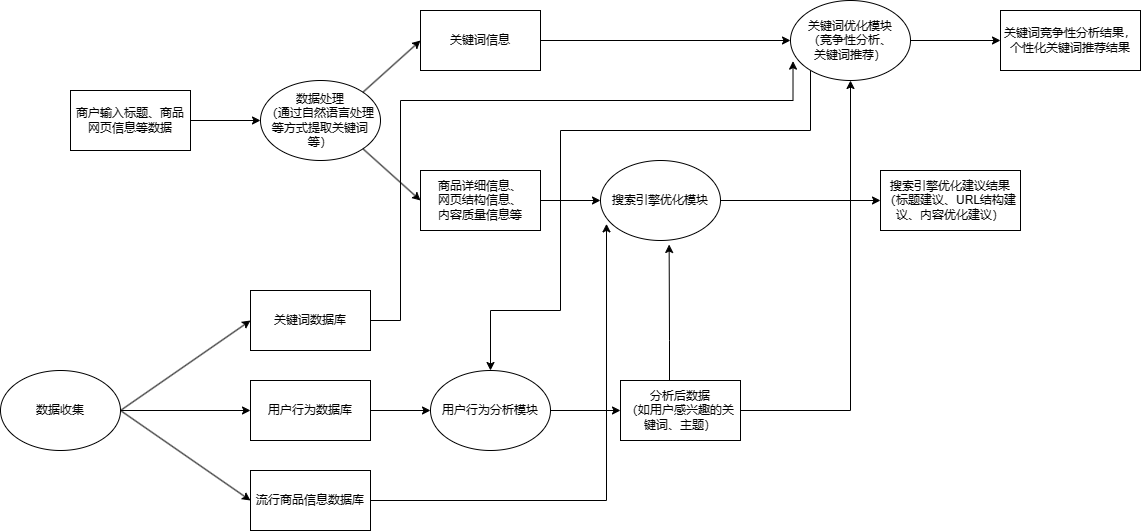
\includegraphics[width=1\textwidth]{系统结构设计1.png}
    \caption{系统结构设计示意图}
    \label{fig:example}
\end{figure}

全系统分为5个子系统:
\begin{enumerate}[itemsep=-5pt]
    \item 数据收集子系统
    \item 输入数据处理子系统
    \item 用户行为分析子系统
    \item 关键词优化子系统
    \item 搜索引擎优化子系统
\end{enumerate}
\section{各子系统功能介绍}
接下来粗略介绍各子系统功能。
\subsection{数据收集子系统}
顶层DFD图:

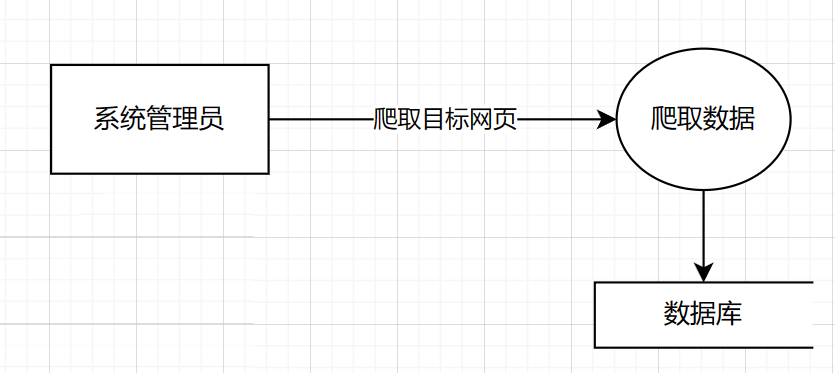
\includegraphics[width=0.75\textwidth]{数据收集系统2_1.png}

功能:
\begin{itemize}
    \item 从互联网上爬取流行商品的网页数据,包括商品标题、描述、关键词等。
    \item 收集用户在电子商务平台上的搜索和购买行为,包括关键词、点击次数、购买次数等。
    \item 提供直接编辑3大数据库的API接口。
\end{itemize}

% 输入:
% \begin{enumerate}
%     \item 流行商品网页URL列表。(爬取列表中网页)
%     \item 用户行为数据。(搜索关键词、点击行为、购买行为)
%     \item 指定(增加)的训练集文件或编辑关键词数据库的操作。
% \end{enumerate}

\subsection{输入数据处理子系统}
顶层DFD图:

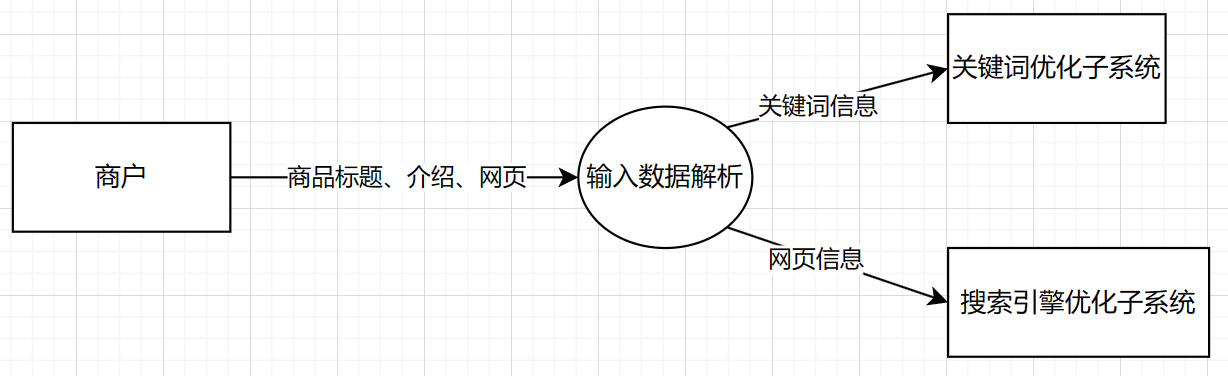
\includegraphics[width=0.75\textwidth]{输入数据解析2_2.png}

功能:
\begin{itemize}
    \item 处理商家输入的商品信息,提取关键词组。
    \item 获取指定商品网页的结构数据和内容数据。
    \item 分析网页内容,生成内容质量数据。
\end{itemize}

% 输入:
% \begin{enumerate}
%     \item 商家输入的商品标题、相关信息
%     \item 商品访问URL
% \end{enumerate}

% 输出:\\[-30pt]
% \begin{itemize}[itemsep=-5pt]
%     \item 关键词优化模块:相关关键词组。
%     \item 搜索引擎优化模块:网页结构数据、网页内容数据、内容质量数据。
% \end{itemize}

\subsection{用户行为分析子系统}
顶层DFD图:

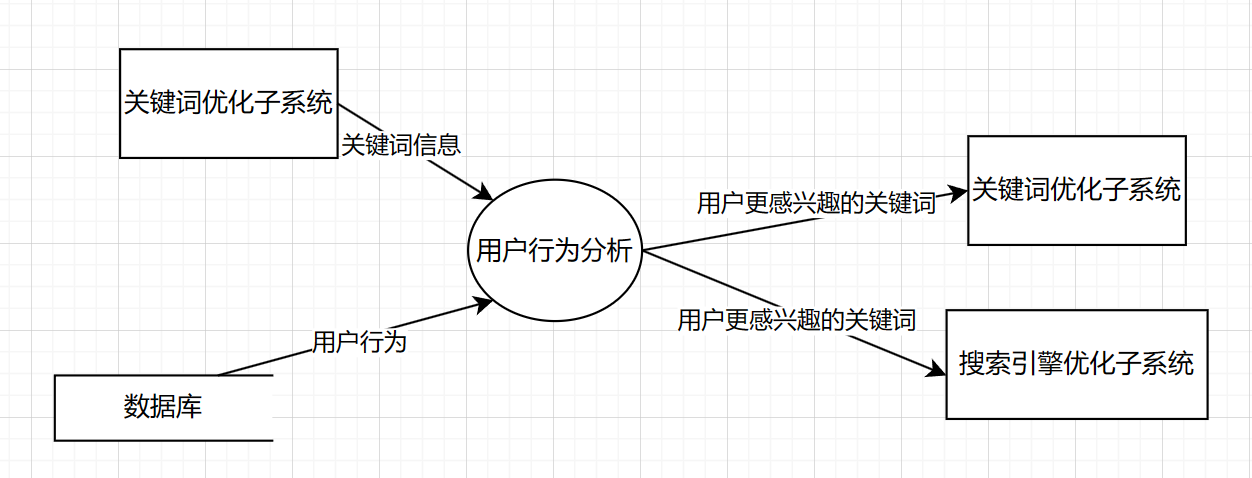
\includegraphics[width=0.75\textwidth]{用户行为分析2_3.png}

功能:分析用户行为数据库和关键词数据库,识别用户感兴趣的商品关键词。
% 输入:
% \begin{enumerate}
%     \item 用户行为数据库
%     \item 关键词数据库
% \end{enumerate}

% 输出:
% \begin{enumerate}
%     \item 用户感兴趣的商品关键词集合
% \end{enumerate}

\subsection{关键词优化子系统}
顶层DFD图:

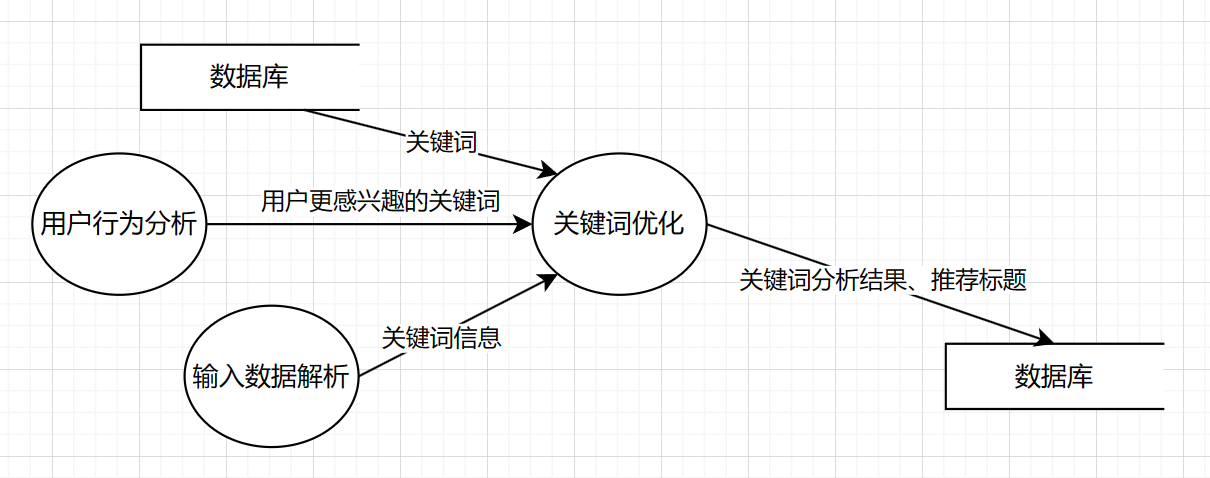
\includegraphics[width=0.75\textwidth]{关键词优化2_4.png}

功能:
\begin{itemize}
    \item 分析商家输入的关键词组和关键词数据库,提供关键词竞争性分析结果。
    \item 提供个性化的关键词推荐结果。
\end{itemize}

\subsection{搜索引擎优化子系统}
顶层DFD图:

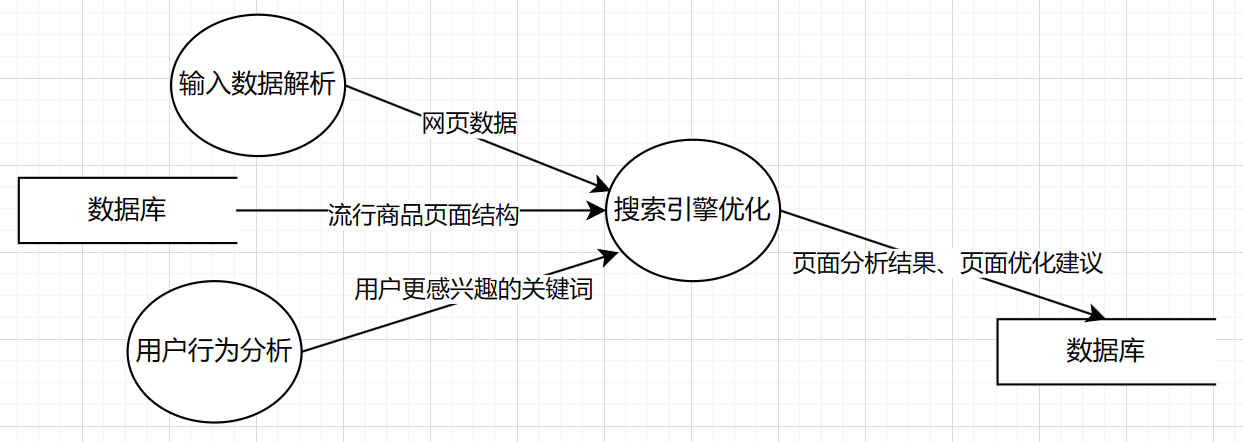
\includegraphics[width=0.75\textwidth]{搜索引擎优化2_5.png}

功能:根据商家的网页内容、网页结构和内容质量数据,提供搜索引擎优化建议结果,包括标题建议、URL结构建议、内容优化建议。

\chapter{功能模块设计}

\section{模块说明}

\subsection{数据收集子系统概要设计}
设计思路:该模块涉及3大数据库生成,将从数据库角度分析实现思路。
\label{chap:chapter3}
\begin{itemize}
    \item 关键词数据库数据生产:关键词数据库将存储$$<\text{关键词}:\text{中介关键词}:\text{竞争关键词}:\text{相关程度}>$$
          每次运行compkey算法将生成一列。鉴于提前生成难度较大,将在每次商家提供商品标题、商品信息,并从中提取关键词组后,再运行compkey算法,并将运行结果存入关键词数据库以备使用。(训练数据集可上传指定,或使用默认训练数据集)
    \item 用户行为数据库数据生成:用户行为数据库将存储$$<\text{用户行为类型(点击/收藏/购买):\text{商品名称}}>$$
          \textbf{使用方式}:提供关键词,查看包含该关键词的所有商品名称的点击/收藏/购买数。

          \textbf{获得方式}:寻找开源数据或爬取购物网站相关数据(商品名+访问次数/销售量/收藏人数)。
    \item 流行商品信息数据库数据生成:该数据库将存储$$<\text{商品名}:\text{网页URL}:\text{商品热度指标}>$$
          \textbf{使用方式}:提供关键词正则,找到商品名符合正则的记录,按热度指标排序,根据URL爬取网页内容和网页结构,以备搜索引擎优化模块的需求。

          \textbf{获得方式}:爬取购物网站热销商品列表,并提取URL,存入数据库。
\end{itemize}

\subsection{输入数据处理子系统概要设计}
该子系统涉及两方面内容,将依次介绍设计思路:
\begin{itemize}
    \item 关键词优化模块:
          \begin{enumerate}
              \item 使用自然语言处理(NLP)技术,可以考虑使用词袋模型(Bag of Words)或者更先进的词嵌入模型(如Word2Vec、BERT)来提取商品名称和介绍中的关键词。
              \item 或利用分词工具对商品名称和介绍进行分词,然后通过关键词提取算法获取关键词。
          \end{enumerate}
    \item 搜索引擎优化模块:
          \begin{enumerate}
              \item URL处理:使用爬虫技术,例如Python中的BeautifulSoup或Scrapy库,来访问商品URL地址并获取网页内容。
              \item 网页结构:使用BeautifulSoup或类似的HTML解析库,遍历HTML文档的标签,获取标签的层次结构和关系。
              \item 内容提取:分析网页结构,可以使用正则表达式或者XPath等方法来提取网页中的关键信息。
              \item 内容质量评价:用自然语言处理(NLP)技术对网页内容进行情感分析,以了解评论或描述的情感倾向;使用模型检测文本的一致性和逻辑性,以评估网页描述的准确性和清晰度。(调用文言一心、GPT等大模型,生成文本、图片的评价,后续可继续调用模型进行文本优化)
          \end{enumerate}
\end{itemize}

\subsection{用户行为分析子系统概要设计}
该子系统可以根据提供的关键词组,返回较受用户青睐的相关关键词组。

设计思路:该模块会被关键词优化子系统所调用,关键词优化子系统会提供一系列与商品关键词相关的关键词组,用户行为分析模块负责使用正则从用户行为数据库中统计与各关键词有关的用户行为数量,并以某类权重公式计算各类型用户行为后,返回<关键词:推荐程度>集合。

\subsection{关键词优化子系统概要设计}
该子系统负责多个功能,将依次介绍设计思路:
\begin{itemize}
    \item 相关关键词组生成:使用Compkey算法,种子关键词为之前输入数据处理模块提取的关键词组,从默认数据集(或指定数据集)中提取出一定数量的中介关键词和竞争关键词,计算关联程度,并存储到关键词数据库;如果数据库已存在该关键词的相关数据库,则直接读取。
    \item 竞争度分析:将竞争关键词和竞争程度返回给用户。如:

          \textit{"手机": "高", "平板电脑": "中", "智能手表": "中"}\vspace{-0.5em}
    \item 关键词推荐:将用户行为分析模块中推荐程度较高的关键词返回给用户。输入输出模拟:

          \textit{输入:}\vspace{-0.5em}

          \textit{\{"推荐关键词": "电脑", "推荐程度": 0.8\},}\vspace{-0.5em}

          \textit{\{"推荐关键词": "游戏", "推荐程度": 0.7\},}\vspace{-0.5em}

          \textit{\{"推荐关键词": "笔记本", "推荐程度": 0.9\},}\vspace{-0.5em}

          \textit{\{"推荐关键词": "性能", "推荐程度": 0.85\}}\vspace{-0.5em}

          \textit{输出:}\vspace{-0.5em}

          \textit{"笔记本", "性能", "电脑"}\vspace{-0.5em}
    \item 商品名称生成:使用GPT、文言一心等大模型,使用固定语法提问,提供原始商品名称、原始关键词、推荐关键词等信息,生成合适的商品名称。输入输出模拟:

          \textit{输入:}\vspace{-0.5em}

          \textit{"原始商品名称": "智能手机",}\vspace{-0.5em}

          \textit{"原始关键词": ["手机", "智能"],}\vspace{-0.5em}

          \textit{"推荐关键词": ["高性能", "全面屏"]}\vspace{-0.5em}

          \textit{输出:}\vspace{-0.5em}

          \textit{"高性能智能手机全面屏版"}\vspace{-0.5em}
\end{itemize}

\subsection{搜索引擎优化子系统概要设计}
该子系统的作用是提供各类搜索引擎优化建议,将依次介绍不同类型建议生成的设计思路:
\begin{enumerate}
    \item 关键词优化建议:
          \begin{enumerate}
              \item 统计网页中的出现的原始关键词、推荐关键词频率、分布,以及提供替代关键词建议。
              \item 密度建议:根据关键词频率和网页总词数,提供关键词密度建议。关键词密度即关键词在文本中的出现次数与总词数的比例。
              \item 分布建议:统计关键词的分布状况,提供关键词在网页中的合理分布建议。避免过度/过少使用关键词,并确保它们自然地融入文本中。
              \item 替代关键词建议:使用了词袋模型和余弦相似度来度量用户提供的关键词与网页内容中其他词的相似度。然后,根据相似度排序,选择了最相似的词作为替代关键词,以丰富网页内容。
          \end{enumerate}
    \item 网页结构优化建议:
          \begin{enumerate}
              \item 标题标签建议:检查每个标题标签的使用情况,并提供建议。可以检查层次结构深度(例如,h2标签应该在h1标签之后使用,h3标签应该在h2标签之后使用)、分布情况(每类标题标签的使用次数,以及它们在文档中的分布),提供建议如:

                    \textit{h1: 没有建议,使用适当。}\vspace{-0.5em}

                    \textit{h2: 建议:调整 h2 标签的层次结构或增加使用频率,以提高合适性。}\vspace{-0.5em}

                    \textit{h3: 建议:调整 h3 标签的层次结构或增加使用频率,以提高合适性。}\vspace{-0.5em}

                    \textit{h4: 建议:添加至少一个 h4 标签以提升页面结构。}\vspace{-0.5em}

                    \textit{h5: 建议:添加至少一个 h5 标签以提升页面结构。}

              \item 段落和文本结构建议:检查段落标签(如p标签)的使用情况,并生成建议。可以检查段落标签(如p标签)和其他文本标签的分布情况、平均段落长度、段落之间的平均间距等,提供建议如:

                    \textit{段落标签\(p\)使用情况: 2}\vspace{-0.5em}

                    \textit{其他文本标签使用情况: 3}\vspace{-0.5em}

                    \textit{建议:}\vspace{-0.5em}

                    \textit{长度建议:某些段落过长,请考虑分割为更短的段落。}\vspace{-0.5em}

                    \textit{标签使用建议:考虑使用更多其他文本标签(如span、div等)来组织文本。}
              \item 图像和多媒体元素建议:检查图像和多媒体元素的使用情况,可以检查是否提供alt属性、图像大小格式等是否合适,并提供建议,如:

                    \textit{建议:图像img\_1缺少描述文本(alt属性),请添加以提高可访问性。}\vspace{-0.5em}

                    \textit{建议:图像img\_2可能过大,请考虑优化图像大小以提高加载性能。}

              \item 链接结构建议:分析页面中的链接结构,检查链接是否具有描述、是否为空链接等。
              \item 页面加载速度建议:分析页面加载速度,提供建议以改善加载性能。如检查是否使用CDN网络、是否使用异步延迟加载、是否使用适当的缓存头(如Cache-Control)、图像格式是否为WebP格式而不是PNG或JPEG等。
          \end{enumerate}
    \item 文本内容优化建议:
          \begin{enumerate}
              \item 根据输入数据处理模块提供的内容质量评价,提示用户修改建议内容;也可继续使用GPT大模型或其他文件优化类模型,生成合适的替换内容以供用户选择。提问方式如:根据以下网页文本信息,根据SEO最佳实践建议,提供语言和内容的优化建议:......
          \end{enumerate}

\end{enumerate}

\section{模块之间的关系}
\subsection{数据收集模块与输入数据处理模块}
\begin{itemize}
    \item 数据收集子系统负责从互联网上爬取流行商品的网页数据,并将其存储到数据库中。
    \item 输入数据处理子系统负责处理商家输入的商品信息,提取关键词组,并获取指定商品网页的结构数据和内容数据。
    \item 数据收集子系统提供的网页数据成为输入数据处理的一部分,用于分析商家输入的商品信息,从而提取关键词组和生成内容质量数据。
\end{itemize}

\subsection{数据收集模块与用户行为分析模块}
\begin{itemize}
    \item 数据收集子系统收集用户在电子商务平台上的搜索和购买行为数据。
    \item 用户行为分析子系统利用数据收集子系统提供的用户行为数据库,分析用户的搜索和购买行为,以识别用户感兴趣的商品关键词。
\end{itemize}

\subsection{输入数据处理模块与用户行为分析模块}
\begin{itemize}
    \item 输入数据处理子系统提供了商家输入的商品信息和相应网页数据。
    \item 用户行为分析子系统结合商家输入的商品信息和用户行为数据,分析用户对商品的兴趣,进一步提供优选关键词。
\end{itemize}

\subsection{关键词优化模块与输入数据处理模块、用户行为分析模块}
\begin{itemize}
    \item 关键词优化子系统分析商家输入的关键词组和关键词数据库。
    \item 输入数据处理子系统提供了商家输入的商品信息和关键词组,而用户行为分析子系统提供了用户对商品的兴趣数据。
    \item 关键词优化子系统综合这些信息,提供关键词竞争性分析和个性化的关键词推荐结果。
\end{itemize}

\subsection{搜索引擎优化模块与输入数据处理模块}
\begin{itemize}
    \item 搜索引擎优化子系统根据商家的网页内容、网页结构和内容质量数据提供优化建议。
    \item 输入数据处理子系统提供了商家输入的商品信息和相应网页数据,为搜索引擎优化提供基础数据。
\end{itemize}

\chapter{数据库设计}
\section{数据库环境}
\textbf{数据库系统}:MySQL 8。

\textbf{设计工具}:Navicat。

\textbf{编程工具}:Navicat提供的SQL编辑器。
\section{数据库表设计}
数据收集模块需要3个表格:
\lstset{
    numbers=left, %设置行号位置
    numberstyle=\tiny, %设置行号大小D:\LaTeX\workspace\homework\软件需求\main.pdf
    keywordstyle=\color{blue}, %设置关键字颜色
    commentstyle=\color[cmyk]{1,0,1,0}, %设置注释颜色
    frame=single, %设置边框格式
    escapeinside=` `, %逃逸字符(1左面的键),用于显示中文
    breaklines=true, %自动折行
    extendedchars=false, %解决代码跨页时,章节标题,页眉等汉字不显示的问题
    xleftmargin=2em,xrightmargin=2em, aboveskip=1em, %设置边距
    tabsize=4, %设置tab空格数
    showspaces=false, %不显示空格
    language=SQL,                                        % 设置语言
}
\begin{lstlisting}
-- ----------------------------
-- Table structure for behavior
-- ----------------------------
DROP TABLE IF EXISTS `behavior`;
CREATE TABLE `behavior`  (
  `id` int NOT NULL AUTO_INCREMENT,
  `behavior` int NOT NULL,
  `commodity` varchar(255) CHARACTER SET utf8mb4 COLLATE utf8mb4_0900_ai_ci NOT NULL,
  PRIMARY KEY (`id`) USING BTREE
) ENGINE = InnoDB CHARACTER SET = utf8mb4 COLLATE = utf8mb4_0900_ai_ci ROW_FORMAT = Dynamic;

-- ----------------------------
-- Table structure for fashion
-- ----------------------------
DROP TABLE IF EXISTS `fashion`;
CREATE TABLE `fashion`  (
  `id` int NOT NULL AUTO_INCREMENT,
  `commodity` varchar(255) CHARACTER SET utf8mb4 COLLATE utf8mb4_0900_ai_ci NOT NULL,
  `URL` varchar(255) CHARACTER SET utf8mb4 COLLATE utf8mb4_0900_ai_ci NOT NULL,
  `degree` float NOT NULL,
  PRIMARY KEY (`id`) USING BTREE
) ENGINE = InnoDB CHARACTER SET = utf8mb4 COLLATE = utf8mb4_0900_ai_ci ROW_FORMAT = Dynamic;

-- ----------------------------
-- Table structure for keyword
-- ----------------------------
DROP TABLE IF EXISTS `keyword`;
CREATE TABLE `keyword`  (
  `id` int UNSIGNED NOT NULL AUTO_INCREMENT,
  `keyword` varchar(255) CHARACTER SET utf8mb4 COLLATE utf8mb4_0900_ai_ci NOT NULL,
  `between` varchar(255) CHARACTER SET utf8mb4 COLLATE utf8mb4_0900_ai_ci NOT NULL,
  `compete` varchar(255) CHARACTER SET utf8mb4 COLLATE utf8mb4_0900_ai_ci NOT NULL,
  `correlation` float NOT NULL,
  PRIMARY KEY (`id`) USING BTREE
) ENGINE = InnoDB CHARACTER SET = utf8mb4 COLLATE = utf8mb4_0900_ai_ci ROW_FORMAT = Dynamic;
\end{lstlisting}

其他表格:
此程序主体只需要上述三个表格,其他表格用于使应用更加完善。表格结构设计已于\ref{chap:chapter3}中介绍。
用户表:
\begin{lstlisting}
-- ----------------------------
-- Table structure for user
-- ----------------------------
DROP TABLE IF EXISTS `user`;
CREATE TABLE `user`  (
  `id` int NOT NULL AUTO_INCREMENT,
  `name` varchar(255) CHARACTER SET utf8mb4 COLLATE utf8mb4_0900_ai_ci NOT NULL,
  `password` varchar(255) CHARACTER SET utf8mb4 COLLATE utf8mb4_0900_ai_ci NOT NULL,
  `usertype` int NOT NULL,
  PRIMARY KEY (`id`) USING BTREE
) ENGINE = InnoDB CHARACTER SET = utf8mb4 COLLATE = utf8mb4_0900_ai_ci ROW_FORMAT = Dynamic;
\end{lstlisting}
结果记录表:
\begin{lstlisting}
    -- ----------------------------
    -- Table structure for result
    -- ----------------------------
    DROP TABLE IF EXISTS `result`;
    CREATE TABLE `result`  (
      `id` int NOT NULL AUTO_INCREMENT,
      `userid` int NOT NULL,
      `keyword\_result` varchar(255) CHARACTER SET utf8mb4 COLLATE utf8mb4_0900_ai_ci NULL DEFAULT NULL,
      `seo\_result` varchar(255) CHARACTER SET utf8mb4 COLLATE utf8mb4_0900_ai_ci NULL DEFAULT NULL,
      PRIMARY KEY (`id`) USING BTREE
    ) ENGINE = InnoDB CHARACTER SET = utf8mb4 COLLATE = utf8mb4_0900_ai_ci ROW_FORMAT = Dynamic;
\end{lstlisting}

\section{数据库结构设计}
% 直接写在这里,两个回车是输出回车
\section{安全性设计}

\subsection{数据保护}

为了确保敏感数据的机密性和完整性,采取以下措施:

\begin{itemize}
  \item 数据库连接采用加密传输,使用 SSL/TLS 协议。
  \item 敏感数据字段采用加密算法RSA进行存储。
  \item 实施备份策略,确保数据定期备份,并存储在安全的地方。
\end{itemize}

\subsection{用户认证和授权}

确保只有授权用户能够访问系统,并按照其角色分配相应权限:

\begin{itemize}
  \item 用户密码存储采用哈希算法,并添加盐以增强安全性。
  \item 实施多因素身份验证,增加用户登录的安全性。
  \item 对用户进行细粒度的授权,限制其访问敏感数据和操作。
\end{itemize}

\subsection{日志记录}

建立全面的日志记录系统,以便监控系统的行为并进行安全审计:

\begin{itemize}
  \item 记录所有用户登录和操作历史。
  \item 使用合适的日志级别,确保能够追踪潜在的安全威胁。
  \item 对日志进行定期审查,及时发现异常或可疑活动。
\end{itemize}

\subsection{防止SQL注入}

通过使用参数化查询或预编译语句等方式,防止SQL注入攻击:

\begin{itemize}
  \item 不直接拼接用户输入到SQL查询中。
  \item 使用ORM(对象关系映射)框架,自动处理参数化查询。
  \item 对输入数据进行严格的验证和过滤,防止恶意输入。
\end{itemize}

\subsection{网络安全}

加强网络安全措施,防范网络攻击:

\begin{itemize}
  \item 使用防火墙限制对数据库的访问。
  \item 定期更新系统和数据库软件,修复潜在的安全漏洞。
  \item 监测和阻止恶意网络流量,例如DDoS攻击。
\end{itemize}
% 直接写在这里,两个回车是输出回车
\chapter{用户界面设计}

\section{搜索页面}

\begin{figure}[h]
  \centering
  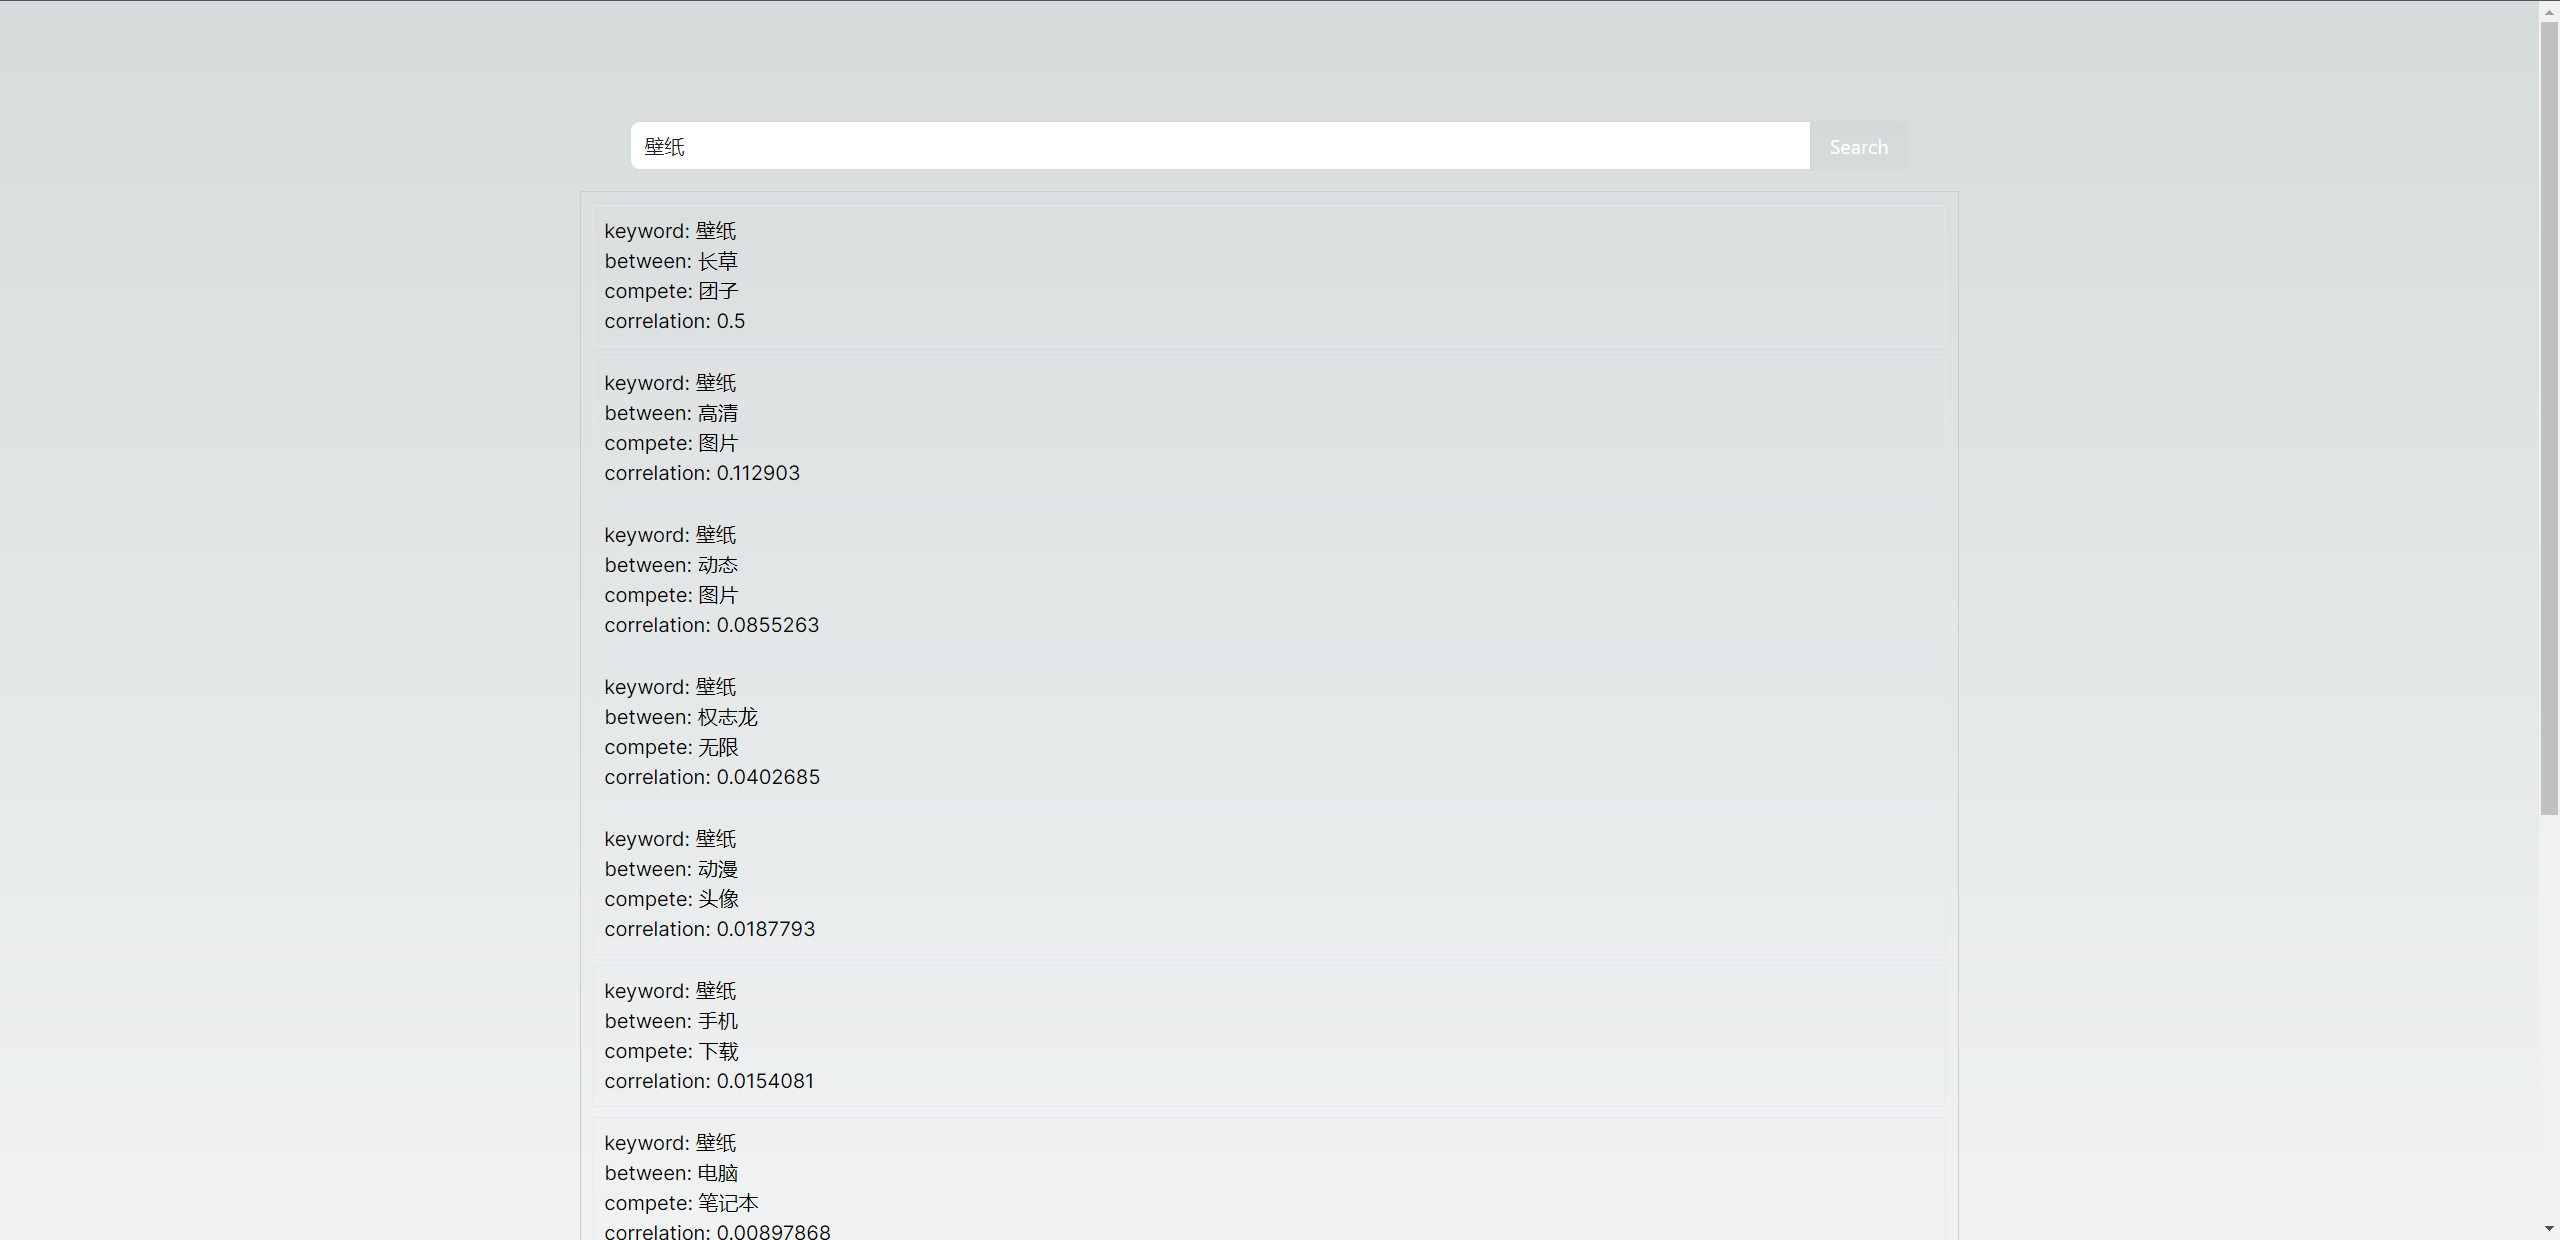
\includegraphics[width=1\textwidth]{运行截图.png}
  \caption{搜索页面}
\end{figure}

\begin{itemize}
  \item **搜索栏:** [文本框] [搜索按钮]
  \item **搜索结果:**
  \begin{itemize}
    \item [结果 1]
    \item [结果 2]
    \item [结果 3]
    % ... 更多搜索结果
  \end{itemize}
\end{itemize}

\section{搜索结果排序}

搜索结果根据竞争度进行排序展示,可以在页面上方或侧边显示排序选项。

\begin{figure}[h]
  \centering
  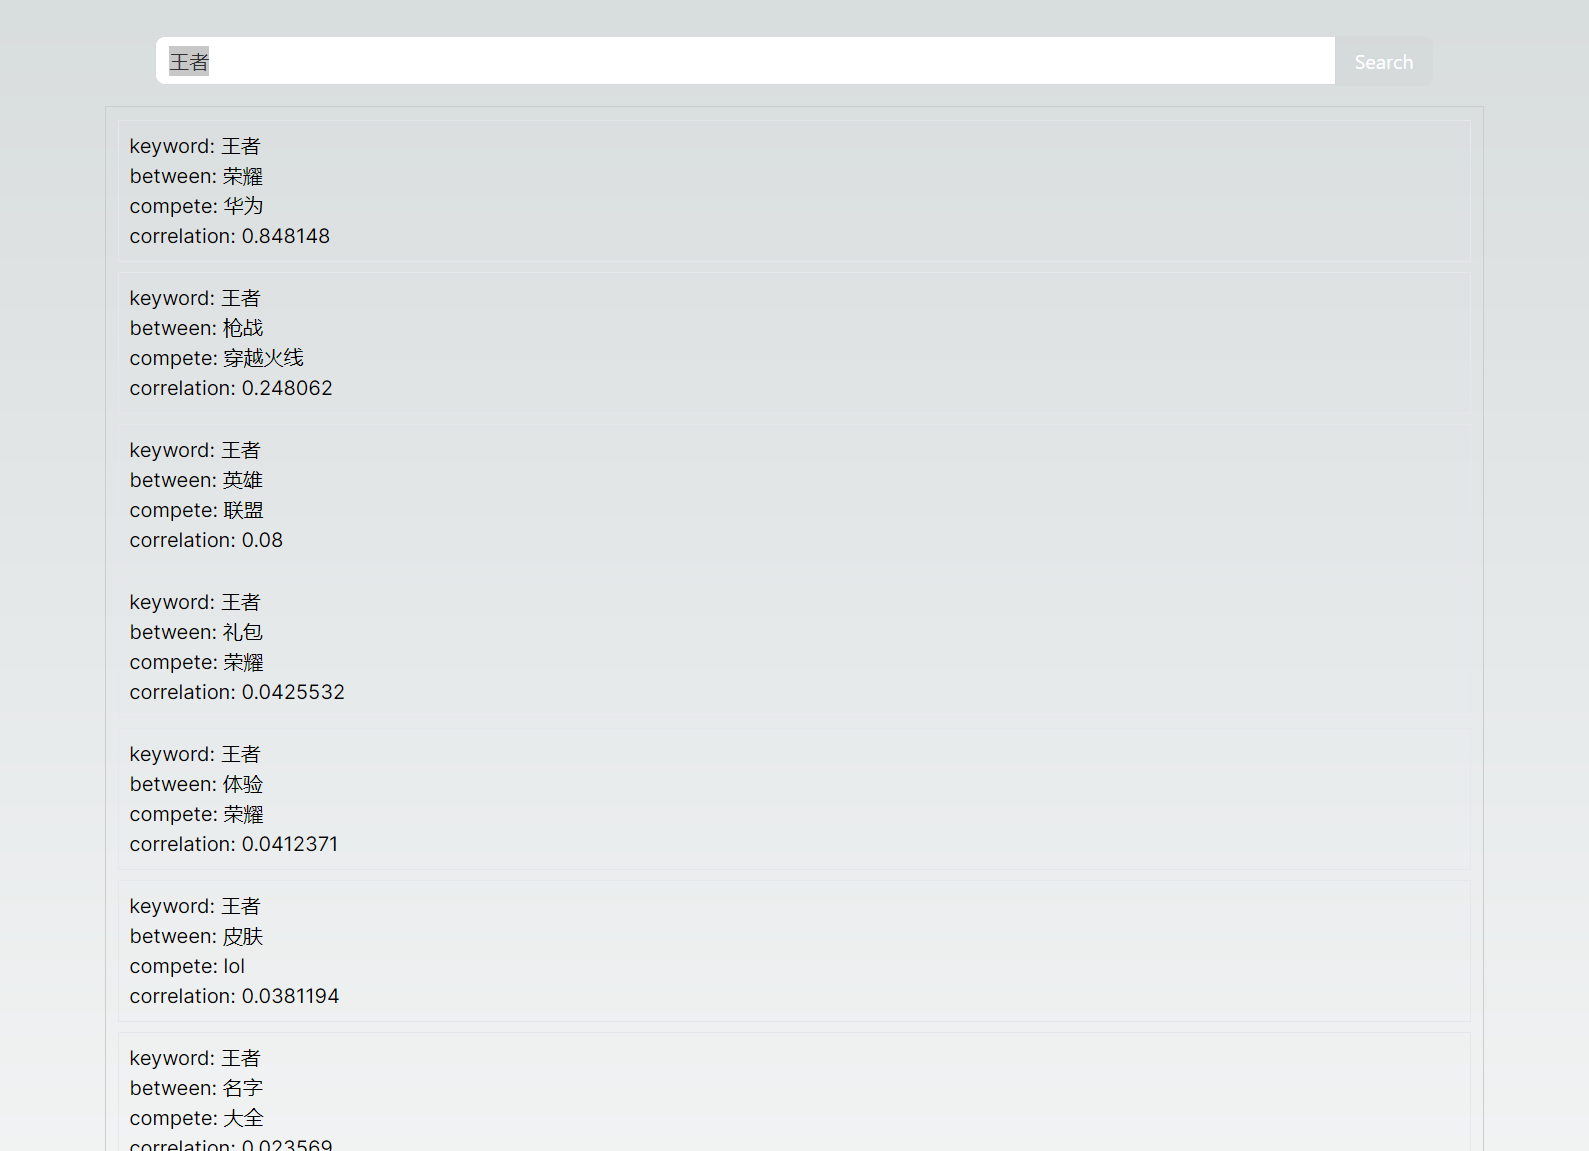
\includegraphics[width=0.8\textwidth]{运行截图2.jpg}
  \caption{搜索结果排序}
\end{figure}

\begin{itemize}
  \item **排序选项:**
   \begin{itemize}
    \item [默认排序]
    \item [竞争度高到低]
    \item [竞争度低到高]
    % ... 其他排序选项
  \end{itemize}
\end{itemize}
\chapter{总结}

电子商务平台SEO推荐系统的核心目标是通过关键词优化和搜索引擎优化,提升商品在搜索结果中的曝光度,以增加用户点击率和购买转化率。系统设计以满足电子商务平台的需求为基础,为商家提供关键词推荐和SEO优化建议,从而最大程度地优化其商品在搜索引擎中的排名。

在本项目中,我们建立了一个综合性的解决方案,包括数据收集模块、用户管理模块和推荐系统。数据收集模块广泛涵盖了用户行为、商品信息和关键词等多个方面的数据,为系统提供了丰富的信息基础。用户管理模块通过用户表和结果记录表,实现了对用户身份的有效管理和对推荐结果的记录。推荐系统充分利用了关键词、商品信息和用户行为等多源数据,通过竞争度排序等策略为商家提供有针对性的SEO优化建议。

通过这个综合性的解决方案,电子商务平台能够更好地理解用户行为、商品特征以及市场竞争状况。商家可以根据系统提供的推荐,有针对性地进行关键词优化和SEO调整,从而提高商品在搜索引擎中的曝光度,吸引更多潜在客户。同时,系统的用户管理模块也为商家提供了用户行为的记录和分析,有助于更好地了解用户需求,提高用户体验。

在未来的发展中,该系统可以通过引入机器学习算法不断优化推荐策略,提高推荐的精准度。同时,随着电子商务行业的不断发展,系统的功能和性能也可以不断升级,以适应不断变化的市场需求。总体而言,电子商务平台SEO推荐系统的实施将为商家带来更为精细化、智能化的运营管理,提升竞争力,实现更好的商业价值。
\end{document}